\documentclass[openany,a4]{book}
%% PAQUETES %%
\usepackage[utf8]{inputenc}
\usepackage{titling}
\usepackage[spanish]{babel}
\usepackage{amsmath}
\usepackage{graphicx}
\usepackage{hyperref}
\usepackage{float}
\usepackage{amssymb}
%\usepackage{ulem}
\usepackage{ragged2e}
\usepackage{fancyhdr}
\usepackage{hyphenat}
\usepackage{titlesec}
\usepackage{wrapfig}


\setlength{\textwidth}{130mm}
\setlength{\textheight}{190mm}
\graphicspath{img/}

%macros
\newcommand{\dpar}[2]{\frac{\partial #1}{\partial #2}}
\newcommand{\prom}[1]{\overline{#1}}
%---------------------------------------------


%% RE ESTILIZACION DE COMNADOS
\titleformat
{\chapter} % command
[display] % shape
{\sc\Large} % format
{Unidad \thechapter} % label
{0.1pt} % sep
{
    \rule{\textwidth}{0.5pt}
    \vspace{0.2ex}
    \centering
} % before-code
\renewcommand{\labelitemi}{$\succ$}
\renewcommand{\chaptermark}[1]{\markboth{\sc #1}{}}
\renewcommand{\chaptermark}[1]{\markright{\sc #1}}

%\fancyhf{}
%\lhead[\thepage]{\rightmark}
%\rhead[\leftmark]{\thepage}
%\renewcommand{\headrulewidth}{0.1mm}
%\renewcommand{\footrulewidth}{0.1mm}

\allowhyphens

\begin{document}


\begin{titlepage}
    \centering
    {\bfseries\LARGE Universidad Nacional de La Plata \par}\vspace{1cm}
    {\scshape\Large Facultad de Ciencias Astronómicas y Geofíscias \par}\vspace{3cm}
    {\scshape\Huge Micrometeorología \par}\vspace{3cm}
    {\itshape\Large Notas teóricas \par}
    \vfill
    {\Large Autor: \par}
    {\Large Lorenzo Girotti \par}
    \vfill
    {\Large 2025 \par}
\end{titlepage}

\sffamily


\chapter{Energía}

\section{Flujos de energía en una superficie ideal}

Consideramos \emph{superficie ideal} a aquella que es relativamente 
suave, horizontal, homogénea, extensiva y opaca a la radiación. 
La energía disponible para tal superficie se simplifica de manera 
tal que solo depende de flujos verticales de energía.

\chapter{Sobre el sistema de ecuaciones}

\section{Ecuación de Navier-Stokes}
Aplicando la segunda ley de Newton y considerando la 
conservación de momento en un volumen elemental de fluido, 
nos lleva a las \emph{ecuaciones de Navier-Stokes}:

\begin{gather}
   \frac{Du}{Dt}-fv=-\frac{1}{\rho}\frac{\partial p}{\partial x}+\nu\nabla^{2}u,\\
   \frac{Dv}{Dt}+fu=-\frac{1}{\rho}\frac{\partial p}{\partial y}+\nu\nabla^{2}v,\\
   \frac{Dw}{Dt}+g=-\frac{1}{\rho}\frac{\partial p}{\partial z}+\nu\nabla^{2}w.
\end{gather}

\par Los primeros términos son los \emph{términos inerciales},
 los segundos representan los \emph{términos de Coriolis} 
 (despreciando Coriolis en la vertical) y la aceleración de la 
 gravedad en la vertical. En el miembro derecho tenemos la 
 fuerza asociada al \emph{gradiente de presión} y \emph{las 
 fuerzas de roce}.

\par Para \emph{fluidos viscosos} necesitamos este set completo de 
ecuaciones que son ecuaciones diferenciales parciales no lineales de 
segundo orden. Prácticamente imposibles de resolver, por lo tanto las 
soluciones analíticas se reservan sólo para casos de flujos laminares 
de baja velocidad.

Sin tensores de Reynolds, es decir, sin considerar turbulencia, tenemos 6
ecuaciones con 6 incógnitas: $u,\,v,\,w,\,p,\,\rho,\,T$

\begin{itemize}
	\item 3 ecuaciones con conservación de cantidad de movimiento:
		$f(u,v,w)$,
	\item 1 ecuación de conservación de masa: $f(\rho)$,
	\item 1 ecuación de conservación de energía: $f(T)$,
	\item 1 ecuación de estado de gases: $f(p)$.
\end{itemize}

\par Cuando incluimos los tensores de Reynolds obtengo un total de 27 variables
nuevas. Por lo cual no es viable cerrar el sistema con más ecuaciones.


\section{Clausura del sistema}
Reemplazamos las tensiones de Reynolds con variables de flujo medio.
Se denomina \emph{clausura del sistema de ecuaciones por flujo turbulento}.

\begin{itemize}
	\item Clausura de primer orden: reemplazo $\prom{u'u'},\prom{u'v'},
\dots$ por variables del flujo medio.
	\item Clausura de segundo orden: retengo las ecuaciones que contienen:
		$\dpar{\prom{u'u'}}{t},\dots$ y reemplazo $\prom{u'u'u'},\dots$ por
		variables de flujo medio.
\end{itemize}
		

\chapter{Flujos}
\section{Definiciones}

\subsubsection{Viscosidad}

Es una propiedad molecular del fluido que representa la resistencia interna del mismo a la deformación. 
En un fluido \emph{ideal} o \emph{no viscoso} se asume un flujo 
no turbulento o laminar, en consecuencia no hay transferencias 
de momento, calor ni masa debido a la mezcla turbulenta; sino 
que las propiedades son transportadas a lo largo de las lineas 
de corriente producto de la advección. Por otro lado, la 
condición de no viscosidad implica que ante la interacción del 
fluido con otro cuya densidad sea significativamente diferente; 
o con una superficie, no habrá fricción entre ellos.

\subsubsection{Fluidos Newtonianos}
La viscosidad es responsable de la resistencia friccional entre capas adyacentes de fluido; la resistencia por unidad de área se llama \emph{tensión por cortante} y se asocia al movimiento relativo entre las capas.

Los fluidos newtonianos son aquellos en donde hay una relación 
proporcional entre la tensión por cortante y el cambio del 
gradiente vertical de velocidad. Donde el coeficiente de 
proporcionalidad $\mu$ se llama viscosidad dinámica del fluido. 
Para flujos se suele utilizar la viscosidad cinemática que es la 
viscosidad dinámica dividido la densidad, con dimensiones de 
$L^2 T^{-1}$.

\subsubsection{Flujos viscosos}

En la realidad siempre existe viscosidad en los flujos. Aún 
así podemos encontrar circunstancias en donde el flujo se 
vuelva \emph{laminar}.

\subsubsection{Flujo laminar}

Se caracteriza por ser suave, ordenado y de movimiento lento, donde 
las capas adyasentes de fluido se deslizan entre sí con muy poca 
transferencia (solo a nivel molecular) de propiedades a través de 
ellas. El campo de flujo, la temperatura asociada y los campos de 
concetración son regulares y predecibles y solo varían gradualmente 
en tiempo y espacio.

\subsubsection{Flujo turbulento}

Son movimientos altamente irregualres, casi aleatorios, 
tridimensionales, altamente rotantes, disipativos y muy difusos 
(mezcla). Todas las propiedades escalares y las del flujo 
fluctuan tanto en tiempo como en espacio, con un amplio rango 
temporal y espacial. Por ejemplo: las fluctuaciones de velocidad en 
la ABL van desde $10^{-3}\mathrm{s}$ a $10^4\mathrm{s}$ y la 
correspondiente al espacio va desde $10^{-3}\mathrm{m}$ a 
$10^4\mathrm{m}$ - del orden del millón en rango. Es por esto 
que es imposible predecir o calcular exactamente a los movimientos 
turbulentos como funciones del tiempo y el espacio; normalmente 
se utilizan los promedios estadísticos de las propiedades.

\subsubsection{Número de Richardson}
\begin{equation}
    \mathrm{Ri}=\frac{g}{T_{v}}\frac{\partial \Theta_{v}}{\partial z}\left|\frac{\partial V}{\partial z}\right|^{-2}
\end{equation}
\par El número de Richardson es una buena medida de la 
turbulencia y provee un criterio simple para la existencia o no 
existencia de turbulencia en un entorno estable estratificado.
\par Un $\mathrm{Ri}>0.25$ indica poco o casi nulo entorno 
turbulento. Por lo tanto, un perfil vertical de $\mathrm{Ri}$ 
deja estudiar con más exactitud la turbulencia en la PBL.

\subsubsection{Número de Reynolds}
\begin{equation}
    \mathrm{Re}=\frac{UL}{\nu}
\end{equation}
donde $U$ es la velocidad característica y $L$ es la longitud de 
escala.

\subsubsection{Longitud de mezcla}
Se define como la distancia que recorre el elemento de fluido hasta que
su cantidad de movimiento equipara a la del medio que lo rodea. $l_z$
es la longitud de mezcla media vertical.

\subsubsection{Coeficiente de intercambio turbulento de cantidad de movimiento $K$.}
\par Se define con unidades dadas por $[K]=L^{2}T^{-1}$ como 
\begin{equation}
    K_{z}=l_{z}^{2}\left|\frac{\partial \bar{u}}{\partial z}\right|
\end{equation}

\section{Ejemplos de distintos escenarios ideales}

\subsection{Flujo laminar entre placas paralelas}
Considerando flujos estacionarios laminares entre dos placas
fijas, paralelas e infinitas; los términos de inercia se cancelan. Además 
para flujos de laboratorio de pequeña escala podemos despreciar
Coriolis, quedando

\begin{figure}[htb]
    \centering
    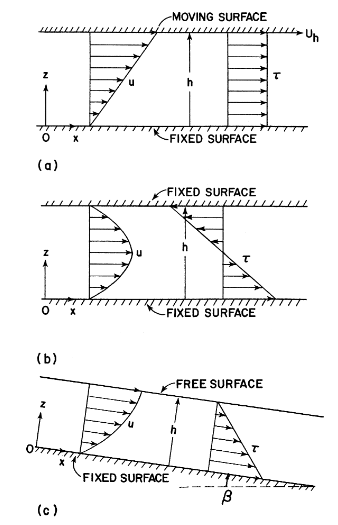
\includegraphics[width=0.6\linewidth]{img/laminar-fluxes.png}
    \caption{(a) Flujo \emph{plane-Couette}; (b) flujo canalizado;
    (c) flujo gravitacional.}
    \label{fig:laminar-flows}
\end{figure}


\begin{equation}
    \frac{d^2u}{dz^2}=\frac{1}{\mu}\frac{\partial p'}{\partial x}
\end{equation}
donde $p'$ es la diferencia entre la presión real y la
hidrostática. Con la suposición de que la densidad sea uniforme,
dicha presión elimina la dependencia de la gravedad. Esto no
puede asumirse cuando la gravedad es un forzante de movimiento,
por ejemplo cuando tenemos un flujo sobre una pendiente.

\subsection{Flujo laminar \textit{plane-Coette}}
Con flujo laminar entre dos placas paralelas, pero en este caso
una es fija y la otra se mueve en la misma dirección que el flujo.
Las condiciones de borde quedan:
\begin{equation}
    \begin{cases}
        u=0,&\quad \mathrm{en}\quad z=0,\\
        u=U_h,&\quad \mathrm{en}\quad z=h.
    \end{cases}
\end{equation}

\par La solución con estas condiciones resulta en una combinación
de perfiles de velocidades lineales y parabólicos.
\begin{equation}
    \frac{u}{U_h}=\frac{z}{h}-\frac{h^2}{2\mu U_h}\frac{\partial p'}{\partial x}\frac{z}{h}\left(1-\frac{z}{h}\right)
\end{equation}

\subsection{Flujo canalizado}
Con el flujo laminar bajo condiciones de borde tales que:

\begin{equation}
    \begin{cases}
        u=0,&\quad \mathrm{en}\quad z=0,\\
        u=0,&\quad \mathrm{en}\quad z=h.
    \end{cases}
\end{equation}

Se obtiene un perfil cuadrático de velocidades:
\begin{equation}
    u=-\frac1{2\mu}\frac{\partial p'}{\partial x}z(h-z).
\end{equation}

\subsection{Flujo gravitacional con pendiente}
Acá consideramos flujo unidireccional con una superficie libre 
u otro flujo gravitacional sobre una superficie uniformemente
inclinada. Considerando una inclinación $\beta$ con respecto a
$x$, tenemos
\begin{equation}
    \frac{d^2u}{dz^2}=-\frac{g}{\nu}\sin{\beta}.
\end{equation}

\par Las condiciones de borde quedan:

\begin{equation}
    \begin{cases}
        u=0,&\quad \mathrm{en}\quad z=0,\\
        du/dz=0,&\quad \mathrm{en}\quad z=h.
    \end{cases}
\end{equation}

\par Nuevamente, obtenemos un perfil cuadrático,
\begin{equation}
    u=\frac{g\sin\beta}{2\nu}z(2h-z).
\end{equation}

En la Figura \ref{fig:laminar-flows} se ven los distintos esquemas
correspondientes a los flujos laminares descritos anteriormente.

\section{Tensiones turbulentas y transporte vertical de cantidad de movimiento}

\chapter{Subcapas de la PBL}
Las alturas promedio de las subcapas en la PBL se pueden ver en la
figura \ref{fig:subcapas-pbl}.
\begin{figure}[htbp]
    \centering
    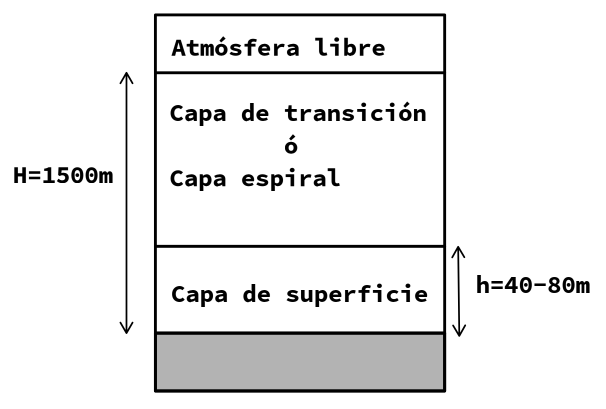
\includegraphics[width=0.8\linewidth]{img/subcapas_PBL.png}
    \caption{Alturas promedio de las subcapas de la PBL.}
    \label{fig:subcapas-pbl}
\end{figure}

En donde $H$ representa la altura en la cual se anula la fuerza de
fricción y $h$ es en donde la \emph{tensión turbulenta} disminuye un
10\% de su valor en la superficie.

\section{Variación del viento con la altura en capa de superficie}
Alineando el eje $x$ en la dirección del movimiento y considerando una
tensión turbulenta constante con la altura, definimos \emph{velocidad
de fricción constante} como

\begin{equation}
    u_{*}^{2}=\frac{\tau}{\rho}>0
\end{equation}

\par Por otro lado, se definió

\begin{equation}
    -\bar{u'w'}=k \frac{\partial u}{\partial z}=u_{*}^{2}
\end{equation}

con $k=l^{2}\left|\partial u/\partial z\right|$, donde $l$ es la
longitud de mezcla.

\par \emph{Prandlt} propuso $l=kz$ siendo $k$ la constante de \emph{Von
Karman} aproximadamente 0.35-0.40. De esta manera se obitiene el
\textbf{perfil logarítimico del viento} (módulo):

\begin{equation}
    u=\frac{u_{*}}{k}\ln{\frac{z}{z_0}},\qquad z_0:\textrm{longitud de rugosidad}
\end{equation}

\par Valores típicos de $z_0$
\begin{itemize}
    \item 0.001m en agua calma o nieve fresca.
    \item 0.01-0.1m en pasto corto.
    \item 1m en bosques.
\end{itemize}
$z_0$ se determina con mediciones del viento a diferentes alturas y se
utiliza reresión lineal.

\section{Variación del viento con altura en la capa espiral}

\section{Capas laminares de Ekman}

\subsection{Capa de Ekman debajo de la superficie del mar}
Ignorando las olas superficiales y los gradientes horizontales tanto
de presión como densidad sobre la superficie; los cambios en las
corrientes justo por debajo de la misma inducidos por un viento
constante siguen estas ecuaciones:
\begin{equation}
    -fv=\nu \frac{d^2u}{dz^2};\quad fu=\nu \frac{d^2v}{dz^2}
\end{equation}

\par Las soluciones dependen de un parámetro $a$ definido por
$a=\sqrt{f/2\nu}$. Teniendo en cuenta la dependencia con el parámetro
de Coriolis, $a\in\mathbb{C}$.

\begin{gather}
    u=(\tau_0/\sqrt{2}a\mu)e^{az}\cos{(az-\pi/4)}\\
    v=(\tau_0/\sqrt{2}a\mu)e^{az}\sin{(az-\pi/4)}
\end{gather}

\par Tenemos entonces una corriente máxima en la superficie ($z=0$)
con un desvío antihorario (acorde a Coriolis en HS) de $45^\circ$. A
medida que la profundidad aumenta ($z<0$), la corriente disminuye su
magnitud y la dirección es cada vez más perpendicular al esfuerzo
superficial inicial.

\begin{figure}[htbp]
    \centering
    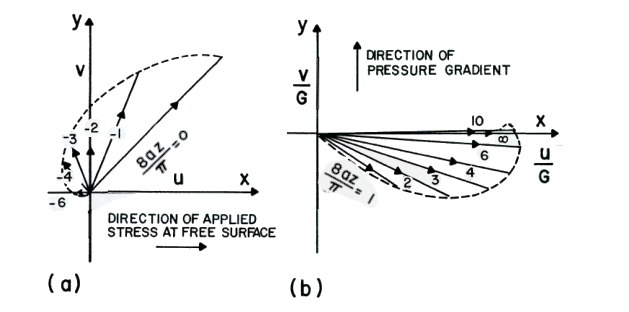
\includegraphics[width=\linewidth]{img/ekman-HS.png} 
    \caption{Hodógrafas: (a) debajo de la superficie del mar; (b)
    encima de una superficie sólida con un gradiente de presión
    constante.}
    \label{fig:ekman}
\end{figure}

\subsection{Capa de Ekman por encima de superficie}
Cuando el aire entra en contacto con un gran cuerpo de agua, o con el
terreno; la fricción desvía el viento del balance geostrófico,
generando así otra espiral de Ekman, esta vez como se muestra en la
Figura \ref{fig:ekman} (b).
\par Asumiendo un gradiente de presión uniforme en las cercanías de
la superficie o en el océano; considerando la superficie plana y
uniforme, y el flujo laminar, las ecuaciones quedan:

\begin{gather}
    -fv=-\frac{1}{\rho}\frac{\partial p}{\partial x}+\nu \frac{d^2u}{dz^2}\\
    fu=-\frac{1}{\rho}\frac{\partial p}{\partial y}+\nu \frac{d^2v}{dz^2}
\end{gather}

\par Expresando los gradientes de presión en términos del viento
geostrófico, las ecuaciones quedan:

\begin{gather}
    -f(v-V_{g})=\nu\frac{d^2(u-U{g})}{dz^2}\\
    f(u-U_{g})=\nu\frac{d^2(v-V_{g})}{dz^2}
\end{gather}

\par Si tomamos al eje $x$ orientado en la dirección del viento
geostrófico, con el módulo $G=\sqrt{U_{g}^2+V_{g}^2}$ la solución 
queda

\begin{gather}
    u=G[1-e^{-az}\cos{(az)}]\\
    v=Ge^{-az}\sin{(az)}.
\end{gather}

\par En la Figura \ref{fig:ekman} (b) podemos observar como el viento
rota de forma antihoraria con la altura.

%----- UTILIZAR LOS APUNTES DE GUILLERMO ------------------
%\paragraph{Altura de la capa de Ekman} 
%\par Está dada por $h_{E}=\pi\sqrt{2\nu/f}$, 
%donde $f\approx 10^{-4}s^{-1}$ la altura es de unos $1.7\mathrm{m}$
%(en el océano la profundidad de la espiral de Ekman es de 
%aproximadamente $0.5\mathrm{m}$)
%##########################################################


\end{document}

